\documentclass{beamer}

\usepackage{amsmath}



\title{Machine Learning in Wireless Communications}
%\subtitle{Markos Loizou\\[7pt]Supervisor: Prof. Ioannis Krikidis}
\author{Markos Loizou\\[7pt]Supervisor: Prof. Ioannis Krikidis}

\usetheme{kios}


\begin{document}
	
	\usebackgroundtemplate{%             declare it
		\tikz[overlay,remember picture] \node[opacity=1, at=(current page.center)] {
			
\includegraphics[height=\paperheight,width=\paperwidth]{presentation_intro.png}};
	}
	
	\frame {
		\titlepage
	}


	\usebackgroundtemplate{%
	
\includegraphics[width=\paperwidth,height=\paperheight]{presentation_background.png}}

	\frame {
		\frametitle{Case Study 1 - Physical Layer Security}
		\framesubtitle{Motivation}
		\vspace{1.5cm}
		\begin{itemize}
			\item<1-> Broadcasting in wireless communications makes it susceptible to eavesdropping.
			\item<2-> Key distribution in dynamic networks used in symmetric crypto-systems.
			\item<2-> High computational complexity of asymmetric crypto-systems.
		\end{itemize}
		\visible<1>{
		\vspace{-2cm}
			\begin{figure}
				\centering
				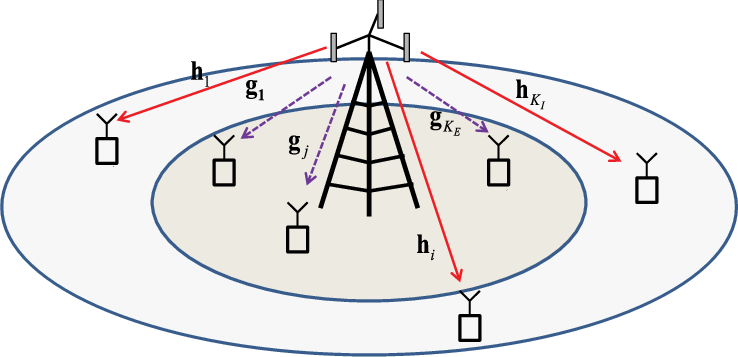
\includegraphics[width = 0.6\paperwidth, height = 0.4\paperheight]{./images/broadcasting.png}
			\end{figure}
		}
	}
	
\begin{frame}
	\frametitle{Case Study 1 - Physical Layer Security}
	\framesubtitle{Information Theoretic Secrecy}
	
	\begin{columns}
	\column{0.5\textwidth}
	\begin{itemize}
		\item The secrecy rate, $C_s$, is the maximum rate which can be transmitted over a communications channel with guaranteed secrecy.
	\end{itemize}
	
	\begin{equation}
		C_s = \left[C^U - C^E\right]^+
	\end{equation}
	
	\begin{itemize}
		\item The channel rate of each user is determined by the channel randomness.
	\end{itemize}
	
    	\column{0.5\textwidth}
		\begin{figure}
		\centering
		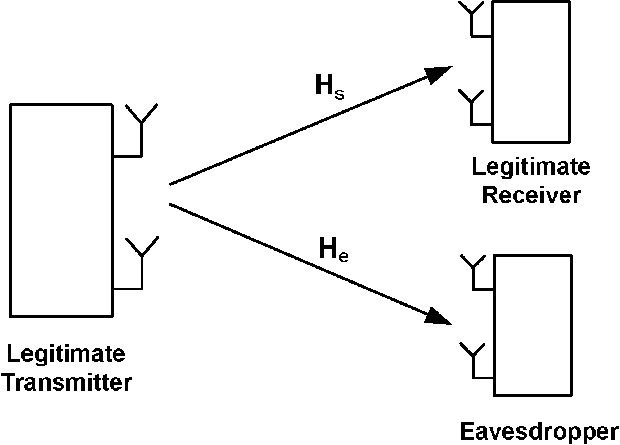
\includegraphics[width = 0.4\paperwidth, height = 0.5\paperheight]{./images/mimome_channel.png}
	\end{figure}
	
	\end{columns}
\end{frame}

\begin{frame}
	\frametitle{Case Study 1 - Physical Layer Security}
	\framesubtitle{MIMO Systems}
	
	
	\begin{itemize}
	    \item MIMO is a technique used to exploit or combat multipath scattering environments. 
	    \item Exploiting them allows for increased throughput.
	    \item Combating  them improves the reliability of communications by exploiting spatial diversity.
	\end{itemize}

\end{frame}

\begin{frame}
	\frametitle{Case Study 1 - Physical Layer Security}
	\framesubtitle{MIMO Systems}
       
    \begin{itemize}
        \item The increased number of antennas also increases their complexity.
        \item By choosing a single antenna, or any subset, we can decrease the complexity. 
        \item Antenna Selection can also be used as a way to increase the security of the system.  
      
    \end{itemize}

\end{frame}

\begin{frame}
    \frametitle{Case Study 1 - Physical Layer Security}
	\framesubtitle{Antenna Selection Techniques}
    
    By choosing a single antenna, $i$, the user receives, 
    
    \begin{equation}
        y^U = H_i^Ux + n^U
    \end{equation} 
    
    and their channel rate (when using MRC) is given by 
    
    \begin{equation}
        R_i = \log_2 \left( 1 + \sum_{j=1}^{N_U} \frac{P \left| h_{ij}^U \right|^2}{\sigma_U^2}\right).
    \end{equation}
    
    
   \begin{itemize}
       \item If only the channel state information, $H$, of the user is known we can chose the antenna that maximizes $R_i$ in hope of also maximizing $C_s$ (SAS).
       \item Another approach is to maximize the smallest singular value of the reduced matrix when selecting a subset of antennas to transmit (MaxMinSV).
   \end{itemize}
             	
\end{frame}
    
    
    
    
\begin{frame}
    \frametitle{Case Study 1 - Physical Layer Security}
	\framesubtitle{Antenna Selection Techniques}
    
    In the case where the eavesdropper is a member of the network and his channel state information is also known, the secrecy rate can be directly maximized by choosing antenna $a$, such that, 
    
    \begin{align}
     a &= \arg\max_i R_s  = \left[R_i^U - R_i^E \right]^+ \\
     &= \arg\max_i \frac{1 + \sum_{j=1}^{N_U} \frac{P \left| h_{ij}^U \right|^2}{\sigma_U^2}}{1 + \sum_{j=1}^{N_E} \frac{P \left| h_{ij}^E \right|^2}{\sigma_E^2}}
    \end{align}
    
    This will be referred to as Optimal Antenna selection (OAS).


\end{frame}


\begin{frame}
    \frametitle{Case Study 1 - Physical Layer Security}
    \framesubtitle{Computational Complexity}
    
    \begin{table}
    \centering
        \begin{tabular}{c|c}
            Selection Method  & Complexity  \\[5pt]
            \hline
            MaxMinSV & $\mathcal{O}(2^{N_t}(N_r N_t^2 + \log(2^{N_t}))$ \\[5pt]
            MaxMinNorm & $\mathcal{O}(\binom{N_t}{N_s}(N_tN_r + \log(\binom{N_t}{N_s})) + N_tN_r)$ \\[5pt]
            OAS & $\mathcal{O}(N_tN_r)$ \\[5pt]
            SAS & $\mathcal{O}(N_tN_r)$ 
        \end{tabular}
    \end{table}
    
   \begin{itemize}
       \item In terms of BER the best Antenna Selection scheme is MaxMinSV which however has a large complexity.
   \end{itemize}
\end{frame}

\begin{frame}
    \frametitle{Case Study 1 - Physical Layer Security}
    \framesubtitle{Machine Learning Algorithms}    
    
    \begin{itemize}
    \item K-Nearest Neighbors (KNN)
    \begin{itemize}
        \item Memory-based with no model to fit
        \item Classifies each point by majority among the k neighbors
    \end{itemize}
    \item Support Vector Machines (SVM)
    \begin{itemize}
        \item Find hyper-planes that give the maximum class separation
        \item Only a \emph{small} subset of the training data is required for classifying new inputs
    \end{itemize}
    \item Multi-Layer Perception Classifier (MLPC)   
    \begin{itemize}
    \item Neural network trained using Adam's Stochastic Optimizer.
    \item Significantly faster training on large data-sets
    \end{itemize}
    \end{itemize}
\end{frame}

\begin{frame}
\frametitle{Case Study 1 - Physical Layer Security}
\framesubtitle{Machine Learning Computational Complexity}
 \begin{table}
     \begin{tabular}{c|c}
         Prediction Method & Complexity \\
        \hline     
         KNN & $\mathcal{O}(N_t N_r)$\\[5pt]    
         SVM & $\mathcal{O}(N_t^2N_r^2)$\\[5pt]
         MLPC &  $\mathcal{O}(N_t^2N_r^2)$
     \end{tabular}
 \end{table}
 \begin{itemize}
     \item All the Machine Learning algorithms have a lower computational complexity for prediction than MaxMinNorm and MaxMinEV
 \end{itemize}
\end{frame}



\begin{frame}
\frametitle{Case Study 1 - Physical Layer Security}
\framesubtitle{Results - Probability of Outage Comparison}

\vspace{-3mm}
\begin{figure}
\centering
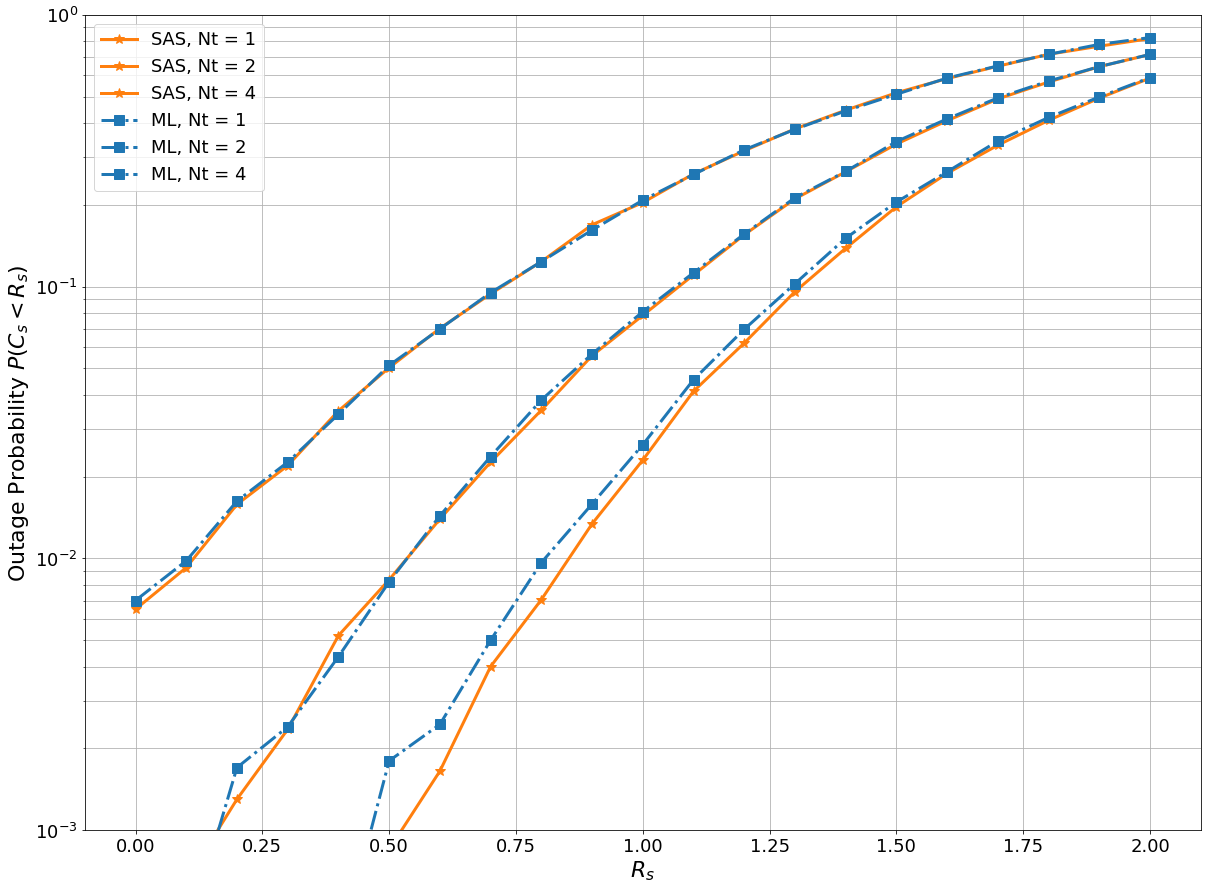
\includegraphics[width=0.7\paperwidth]{./images/outage_sas.png}
\end{figure}
    \vspace{-7mm}
    \begin{itemize}
        \item The machine learning algorithms perform as well as the analytic techniques (Nr = 10 for this example).
    \end{itemize}
\end{frame}


\begin{frame}
    \frametitle{Case Study 1 - Physical Layer Security}
    \framesubtitle{Results -  Imperfect CSI  Antenna Selection}
    \vspace{-3mm}
    \begin{figure}
        \centering
        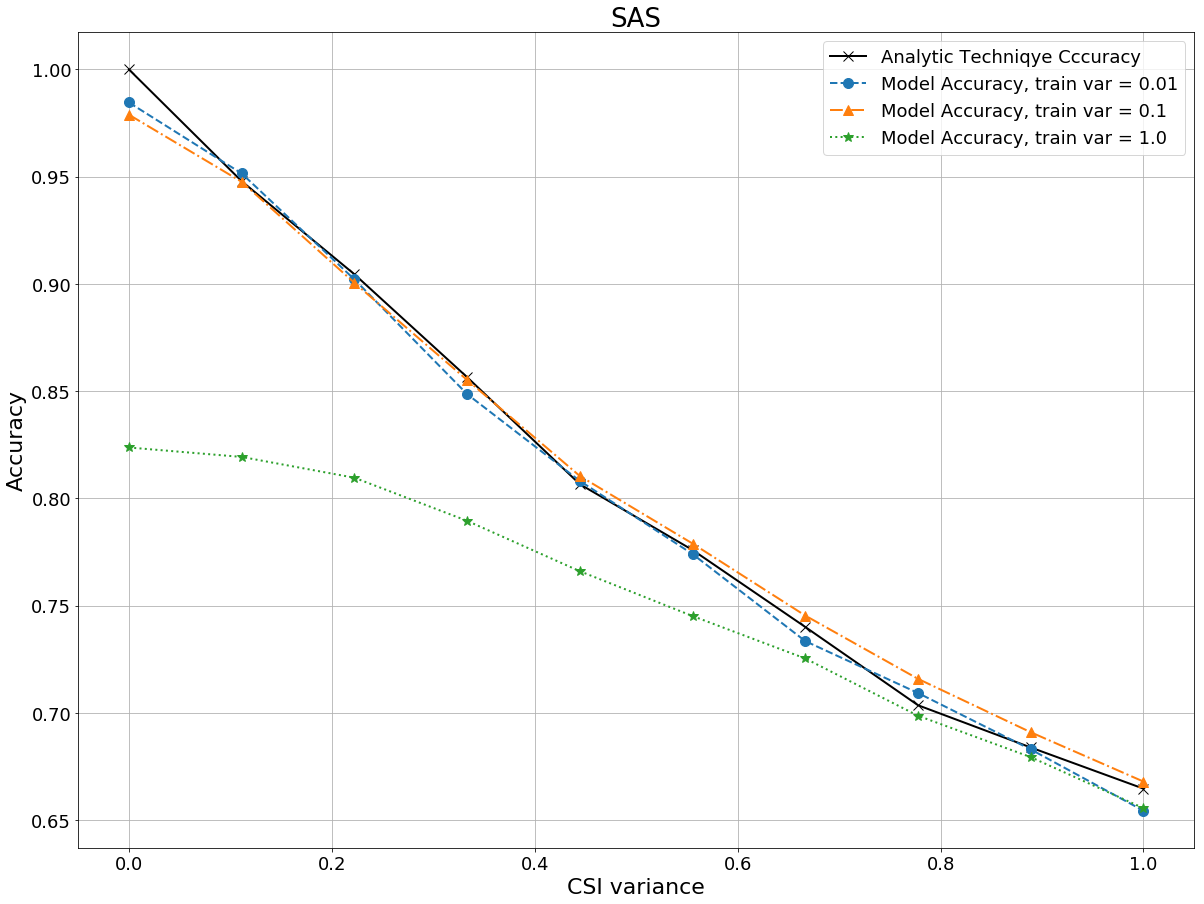
\includegraphics[width = 0.7\paperwidth]{./images/csi_sas.png}
    \end{figure}
    \vspace{-6mm}
     \begin{itemize}
         \item Machine learning algorithms are as robust to noise as the traditional techniques.
     \end{itemize}

\end{frame}

\begin{frame}
    \frametitle{Case Study 2 - RF for Detection}
    \begin{itemize}
        \item Traditionally Radio Frequency waves have only been used for transmitting information.
        \item More recently, RF waves have also been investigated to transmit power for energy harvesting devices.  
        \item A new application of RF is for detection and classification of objects and events. 
        \item The received signal carries information about the channel (environment) the waves propagated through. This information can be used for detection.
    \end{itemize}
    
    \visible<2->{
    \begin{footnotesize}
        A recent paper used two WiFi modules connected on two laptops to identify with high accuracy the quality of wheat. Traditional techniques require expensive equipment, trained personnel while having similar accuracy.
        
        Related work has also been done on WiFire and WiMetal, where RF waves were used to detect fire events and metal object respectively. 
    \end{footnotesize}
    }
\end{frame}

\begin{frame}
    \frametitle{Case Study 2 - RF for Detection}
    \framesubtitle{Method}
    
    \begin{itemize}
    \item A USRP was used to transmit a sine wave. 
    \item An object was placed between the transmitter and the receiver (at 3 locations). 
    \item The receiver recorded the amplitude and phase of the received signal. 
    \item The received signal was used to classify the two objects. 
    \item The two objects used were glasses(glass, plastic and metal) and planar objects (mirror, plastic, metallic, wooden).
    \item We then classified the objects into glasses and planar objects. 
    \end{itemize}
\end{frame}

\begin{frame}
    \frametitle{Case Study 2 - RF for Detection}
    \framesubtitle{Setup}
    \begin{figure}
        \centering
        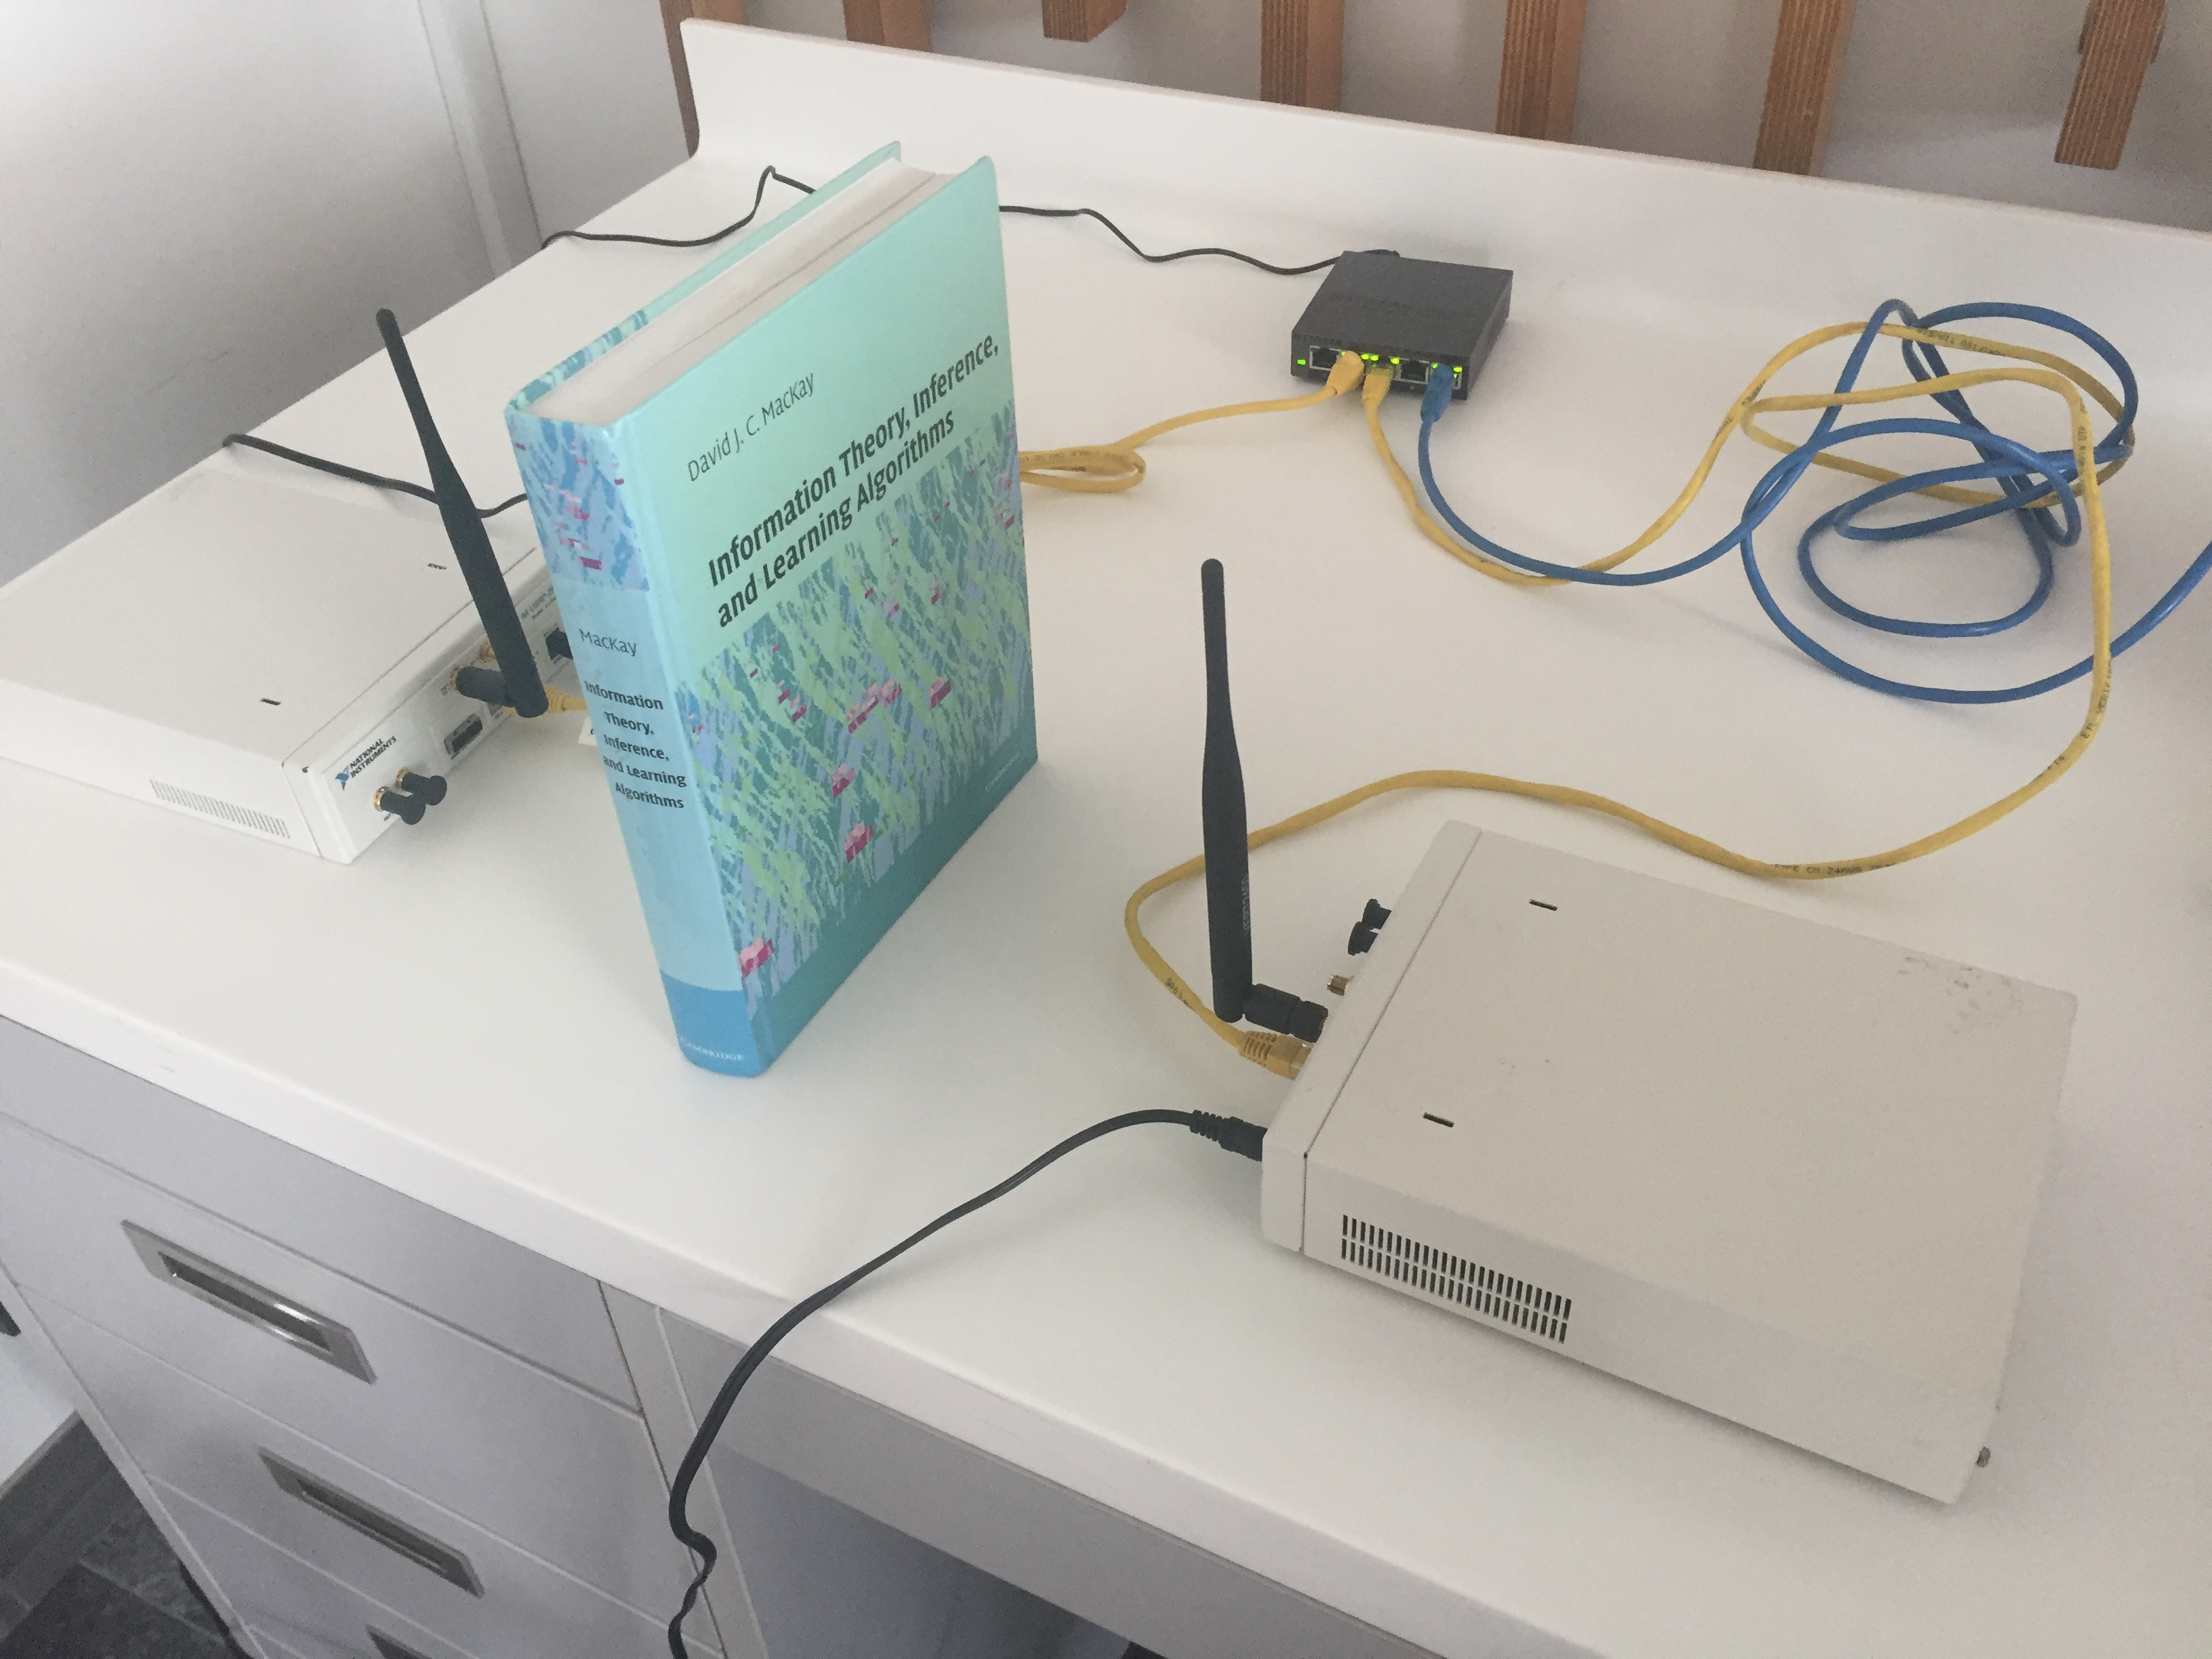
\includegraphics[width=0.8\paperwidth]{./images/usrp2.JPG}
    \end{figure}
\end{frame}

\begin{frame}
    \frametitle{Case Study 2 - RF for Detection}
    \framesubtitle{Data Preparation and Training}
    
    \begin{itemize}
    \item The start and end of the signal were discarded since no signal was transmitted at those times. 
    \item Each measurement(12000 sample points) was broken into smaller ones, each one containing about 1 period of the wave(200 sample points)
    \item Complex data was transformed into magnitude and phase.
    \item The data was then normalized to lie in $[0,1]$.
    \item The data was then labeled with class 0 for glasses and 1 for the planar objects. 
    \item The same supervised learning algorithms as before were trained using part of the labeled dataset. 
    \item The most promising model was then tested on the remaining dataset.
    \end{itemize}
\end{frame}

\begin{frame}
\frametitle{Case Study 2 - RF for Detection}
\framesubtitle{Results}
\begin{itemize}
\item<1-> \emph{The MLPC achieved 95\% accuracy}
\end{itemize}
\vspace{-0.3cm}
\visible<2->{
\begin{figure}
\centering
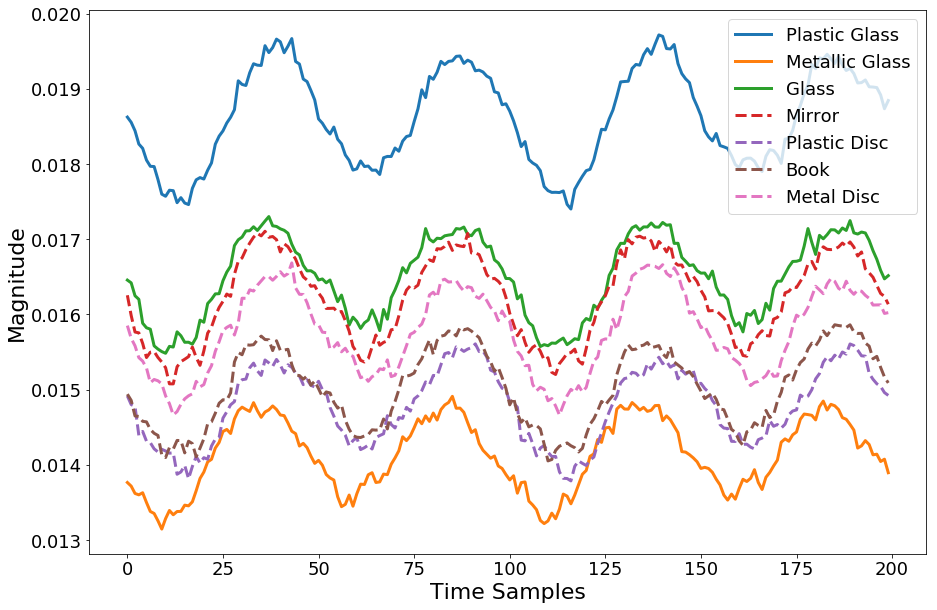
\includegraphics[width = 0.9\textwidth]{./images/objects.png}
\end{figure}
}
\end{frame}

\begin{frame}
    \frametitle{Further Work}
    
    \begin{itemize}
        \item Use Reinforcement Learning for antenna selection.
        \item Use Reinforcement Learning for jamming as well as selecting the transmit antenna.
        \item Classify materials as well as objects.
        \item Make the predictions in real time. 
    \end{itemize}
\end{frame}

\begin{frame}
    \frametitle{Conclusions}
    
    \begin{itemize}
    \item Machine Learning can be useful in Wireless Communications for:
	    \begin{itemize}
	    \item Lowering computational complexity.
	    \item Tackling problems with no known solutions.
	    \item Tackling problems with no models.
	    \end{itemize}
    \end{itemize}
\end{frame}


\begin{frame}
\centering
\Huge{\color[RGB]{204,0,0}Thank You!}
\end{frame}

\end{document}